\documentclass[a4paper]{article}
\usepackage[top=1in, bottom=1in, left=1in, right=1in]{geometry}
\usepackage{amsmath}
\usepackage{amsfonts}
\usepackage{amssymb}
\usepackage{booktabs}
\usepackage{graphicx}
\usepackage{enumerate}
\usepackage{xeCJK}
\usepackage{zhnumber}
\usepackage{listings}
\usepackage{float}
\usepackage{multirow}
\usepackage[colorlinks,linkcolor=black,anchorcolor=black,citecolor=black]{hyperref}
\setCJKmainfont[BoldFont=Source Han Serif CN SemiBold]{Source Han Serif CN}
\setCJKfamilyfont{hei}{Source Han Sans CN}
\setCJKfamilyfont{kai}{Source Han Sans CN}
\setCJKfamilyfont{fang}{Source Han Sans CN}
\newcommand{\hei}{\CJKfamily{hei}}
\newcommand{\kai}{\CJKfamily{kai}}
\newcommand{\fang}{\CJKfamily{fang}}

\usepackage{fontspec}
\newfontfamily\mymono{Source Code Pro}
\usepackage{color}
\definecolor{mygreen}{rgb}{0,0.6,0}
\definecolor{mygray}{rgb}{0.5,0.5,0.5}
\definecolor{mymauve}{rgb}{0.58,0,0.82}
\lstset{
	frame=none,
	numbers=none,
	numberstyle=\footnotesize\mymono\color{mygray},
	basicstyle=\footnotesize\mymono,
	breaklines=true,
	tabsize=4,
	commentstyle=\color{mygreen},
	keywordstyle=\color{blue},
	stringstyle=\color{mymauve},
}

\newcommand{\tabincell}[2]{\begin{tabular}{@{}#1@{}}#2\end{tabular}}

\title{机器学习概论课程实验报告\\\textit{Fake News Detection}}
\author{孟垂正\footnote{学号: 2013010952, 邮箱: mengcz95thu@gmail.com, 电话: 17600739085.}}
\date{\zhtoday}

\begin{document}
	\maketitle\thispagestyle{empty}
	\renewcommand{\contentsname}{目录}
	\tableofcontents
	\clearpage
	
	\setcounter{page}{1}
	\section{问题介绍}
	该问题来源于比赛Fake News Challenge\footnote{http://www.fakenewschallenge.org/}. 比赛的目标是利用人工智能技术提高检测一个消息是否为谣言的工作的自动化程度, 减轻人类审查员的负担. 本次挑战并没有打算一劳永逸地自动化全部的检测步骤, 而是试图完成其中比较重要的一个步骤--Stance Detection, 即检测不同的媒体对于同一个话题的态度. 很显然如果他们的态度相差很大或者负面态度居多, 该消息的可信性将大打折扣. 这一步工作将成为未来的自动谣言检测系统的重要组成部分之一.

	\section{相关工作}
	本次需要解决的问题属于stance detection问题, 即给出2段文本, 判断它们表达的观点是否一致. 类似的问题之前也被数次提出过并作为一些比赛的题目. 例如2016年的SemEval-Task 6要求参赛者判断给出的twitter文本是否支持其所属的主题, 并需要完成有监督/无监督2种情形下的任务\cite{mohammad2016semeval}. 在该比赛中深度学习的模型得到了广泛的应用, 分获第一名和第二名的2支队伍分别使用了RNN\cite{zarrella2016mitre}和CNN\cite{wei2016pkudblab}解决该问题.\\\\
	Stance detection问题是文本分类问题的一种, 目前已有较多使用RNN等模型完成文本分类任务的工作发表, 例如使用双向RNN进行分类\cite{graves2005framewise}, 使用RNN与CNN的混合模型进行文本分类\cite{lai2015recurrent}, 以及使用引入attention机制的RNN模型进行分类\cite{luong2015effective}\cite{chen2016thorough}.\\\\
	与传统的提取特征的方法相比, 以上的深度学习模型要求将文本转化为数值向量后输入模型进行计算, 即需要进行合适的word embedding. 这一领域的工作有Mikolov等提出的word2vec\cite{mikolov2013distributed}, Pennington等提出的GloVe\cite{pennington2014glove}和Bojanowski等提出的Fasttext\cite{bojanowski2016enriching}.
	
	\section{实验任务}
	实验需要完成的任务是: 在比赛方提供的有标注数据基础上构建模型, 判断消息正文与消息标题之间的关系, 包括同意, 反对, 不表态, 无关四种. 具体如下:
	\begin{itemize}
		\item 输入: 一个标题和一段正文(二者可能来自同一个消息也可能不是).
		\item 输出: 标题与正文的关系, 分为以下4类:
		\begin{itemize}
			\item Agrees: 正文内容同意标题内容;
			\item Disagrees: 正文内容反对标题内容;
			\item Discusses: 正文与标题讨论了同一个话题, 但没有表明态度;
			\item Unrelated: 正文与标题讨论的话题不同.
		\end{itemize}
	\end{itemize}
	数据来源是比赛方提供的有标注数据\footnote{https://github.com/FakeNewsChallenge/fnc-1}, 规模在50k篇文章左右, 包含了标题, 正文以及标题和正文之间的关系.
	
	\section{模型设计}
	\subsection{Baseline}
	Baseline模型来源于数据提供方\footnote{https://github.com/FakeNewsChallenge/fnc-1-baseline}. 该模型从标题和正文中手工提取特征, 然后使用Gradient Tree Boosting Classifier进行分类.\\\\
	提取的特征包括:
	\begin{itemize}
		\item word overlap features: 标题和正文词汇的Jaccard相似度\cite{niwattanakul2013using}.
		\item refuting features: 由 refuting words 在标题中的出现情况组成的0-1向量. Refuting words包括'fake',
		'fraud',
		'hoax',
		'false',
		'deny', 'denies',
		'not',
		'despite',
		'nope',
		'doubt', 'doubts',
		'bogus',
		'debunk',
		'pranks',
		'retract'. 若某个词在标题中出现则对应位置为1, 否则为0.
		\item polarity features: 标题和正文表现出的态度的"极性". 一段文本的"极性"的计算方法是统计前述refuting words在其中出现次数的奇偶性. 偶数次的否定体现出肯定的态度, 奇数次的否定则仍旧体现出否定态度.
		\item binary co-occurrence: 标题中的词汇在正文中出现的次数总和.
		\item binary co-occurrence stops: 除去stop words(一些无实际意义的词汇, 例如a, the, is等)的标题中的词汇在正文中出现的次数总和.
		\item count grams: 标题中n个连续字母/n个连续单词在正文中出现的次数, 对于字母, 模型选取了n=2,4,8,16; 对于单词, 模型选取了n=2,3,4,5,6.
	\end{itemize}
	分类器使用决策树作为基分类器, 同时使用Gradient Boosting方法\cite{friedman2002stochastic}作为增强学习方法. Gradient Boosting方法与Boosting方法执行流程类似, 均为串行执行, 但前者每次更新时使用损失函数对分类结果的梯度而非真实结果训练新的基分类器, 并确定一个使得更新后损失结果最小的步长, 本轮更新后的分类结果为上一轮的结果+步长*本轮基分类器的结果. Gradient Boosting的优势是预测能力较强, 缺点是不便于并行化.
	\subsection{Word Embedding}
	大多数机器学习方法更擅长处理数值类型的输入数据, 因此有必要使用word embedding将输入文本中的单词映射为n维向量. 一个好的word embedding应当将语义相近的词汇映射到n维空间的相近位置, 同时词向量之间的位置关系应当能较好地反应原词汇之间的关系. 考虑到本实验中可用数据较少, 直接使用预训练的模型效果更好. \\\\
	综合考虑各个预训练模型的大小, 特征维数和使用的数据集大小, 本实验选择Stanford NLP Group在twitter数据集上训练的的GLoVe模型\footnote{http://nlp.stanford.edu/data/glove.twitter.27B.zip}作为word embedding. 该模型包含1.2百万个单词, 结果为25/50/100/200维的词向量.
	\subsection{损失函数}
	对于神经网络模型, 需要选择合适的损失函数以进行参数求导和优化. 这里选择的损失函数为分类问题中常用的Cross Entropy函数, 该函数的形式如下:
	\begin{equation*}
		L(X,Y)=-\sum_{n}\sum_{i}y_i^{(n)}\log{(f(x^{(n)})_i)}
	\end{equation*}
	其中$y_i^{(n)}$为二值函数, 表示第n个样本的真实类别是否为$i$, $f(x^{(n)})_i$为模型输出的将第n个样本预测为$i$类的概率. 可以观察到$e^{-L(X,Y)}$实际上就是模型将输入$X$分类到$Y$的概率, 因此对该损失函数求极小相当于进行了极大似然估计.
	\subsection{基于CNN的模型}
	\begin{figure}[H]
		\centering
		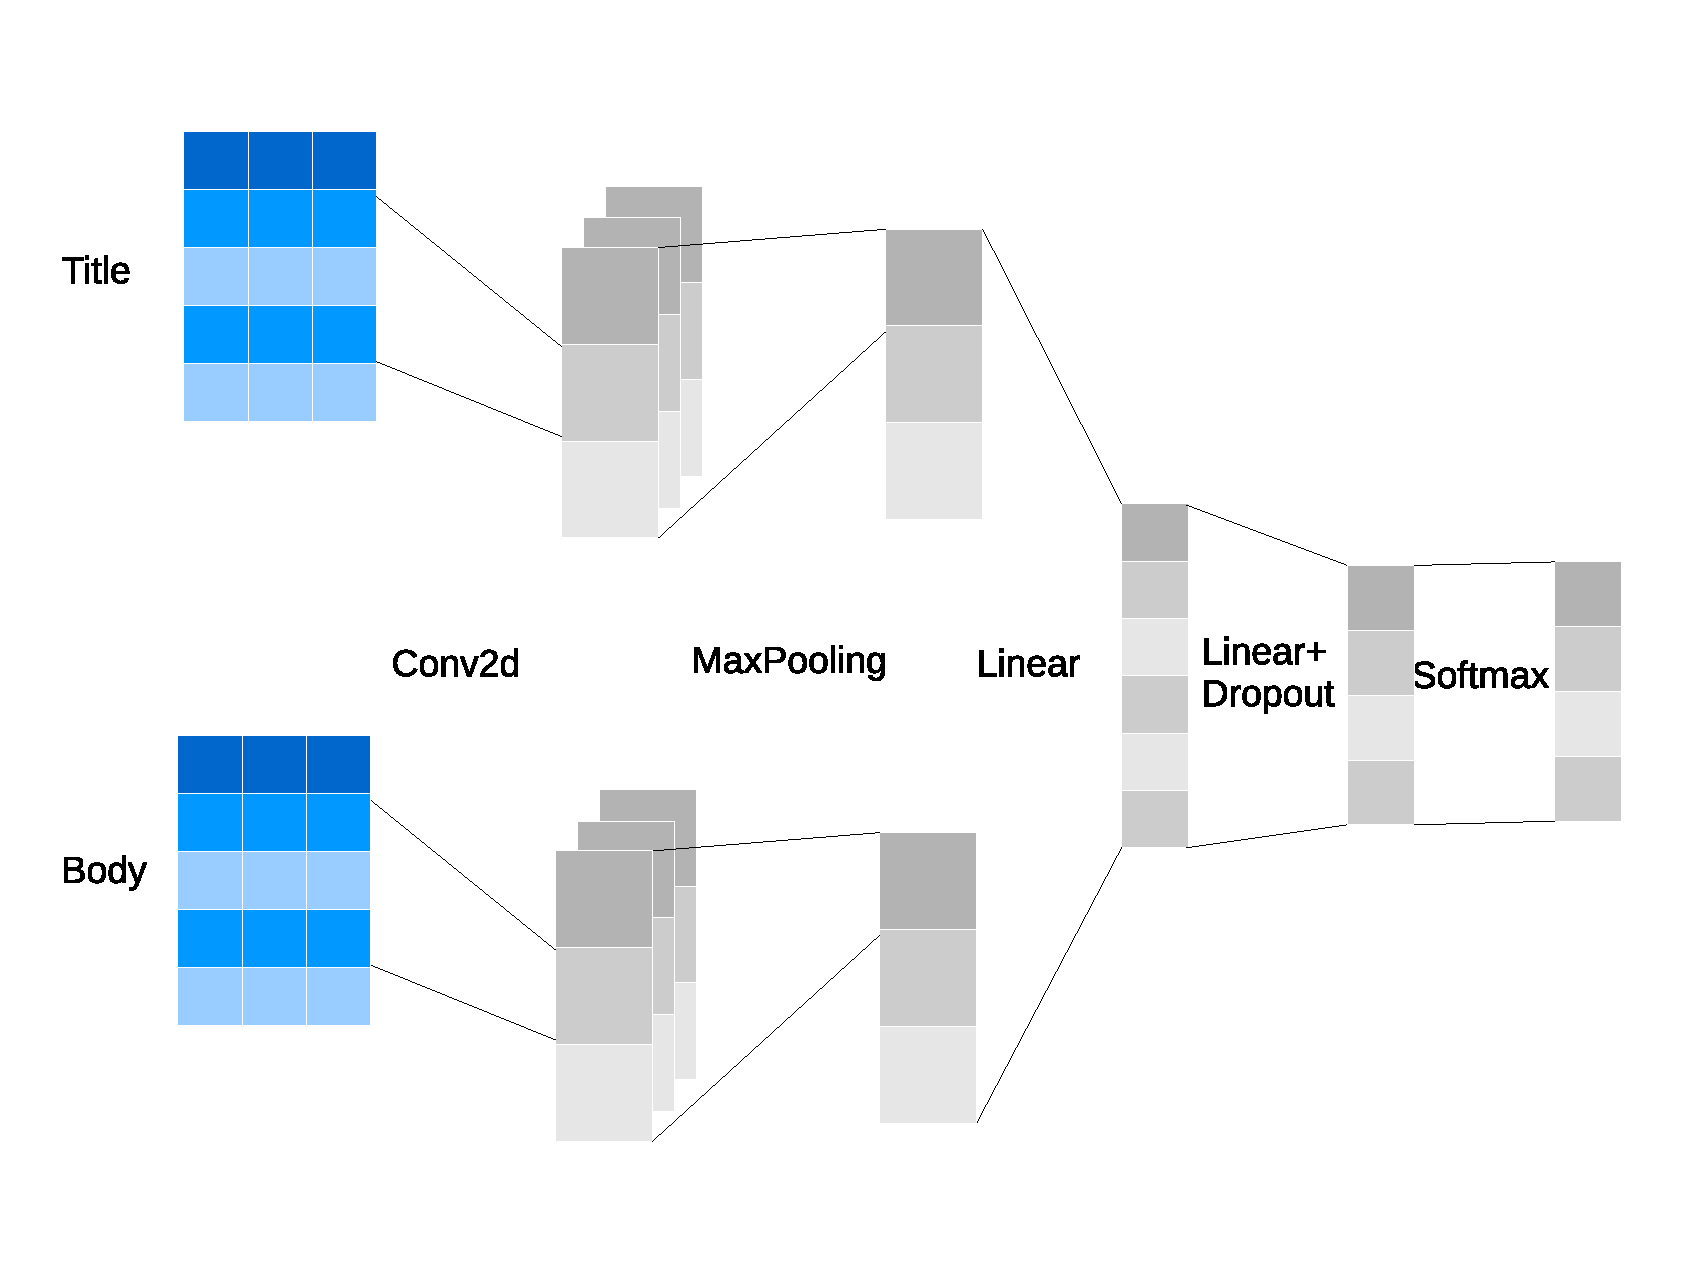
\includegraphics[width=0.8\textwidth]{cnn.eps}
		\caption{用于分类的CNN模型示意图, 包括卷积, 池化, 线性层和softmax层}
		\label{cnn}
	\end{figure}
	CNN全称为卷积神经网络(convolutional neural network), 该网络通过引入卷积核实现了对局部特征的提取, 同时减少了模型的参数数量. 在文本分类任务中, 卷积核可以在一定程度上捕捉上下文之间的词汇关系. 本实验用于文本分类的CNN模型组成部分主要有:
	\begin{itemize}
		\item word2vec: 将标题/正文文本通过预训练的word2vec模型转化为输入矩阵, 大小为文本长度x词向量维数.
		\item 卷积层: 卷积核大小为窗口大小x词向量维数, stride为1, 不进行padding. 标题文本卷积核数量与词向量维数相同. 对于标题文本窗口大小为3, 对于正文窗口大小为5.
		\item 池化层: 使用MaxPooling, 对每个卷积核的结果取最大值.
		\item 线性层: 将title和body文本经过卷积池化的结果拼接后输入线性层, 得到隐层结果.
		\item 线性层+Dropout层: 将隐层结果输入线性层得到长度为4(类别数)的输出层. 对隐层的结果进行一定概率(0.1)的dropout操作, 即使得该层神经元的输出在训练时有0.1的概率为0, 在预测时恢复正常, 可以抑制过拟合现象的发生\cite{srivastava2014dropout}.
		\item Softmax层: 将输出层的结果输入softmax函数得到最终分类结果, 输出样本属于4种类别的概率.
	\end{itemize}
	\subsection{基于RNN的模型}
	RNN全称为循环神经网络(recurrent neural network), 该网络要求输入数据按照一定序列进入网络, 时刻t输入的数据包括序列中的第t个数据和t-1时刻的网络输出结果. 这一特点使得RNN具有一定的记忆功能, 适合处理文本等序列数据, 因此RNN模型在自然语言处理领域得到了广泛的应用. 输入序列较长时RNN"记忆"的向量会出现衰减现象, 但2种特殊的RNN单元LSTM\cite{gers2000learning}和GRU\cite{chung2014empirical}的提出解决了这一问题. 以下的模型均使用LSTM/GRU作为网络基本单元.\\\\
	下面几种RNN模型的区别主要在于RNN部分, 分类部分均使用有1个隐层的线性网络+softmax进行分类, 同时对隐层做dropout处理抑制过拟合.\\\\
	文本序列均经过GLoVe模型转换为词向量序列, 为简便未在图中画出.
	\subsubsection{双向RNN模型}
	\begin{figure}[H]
		\centering
		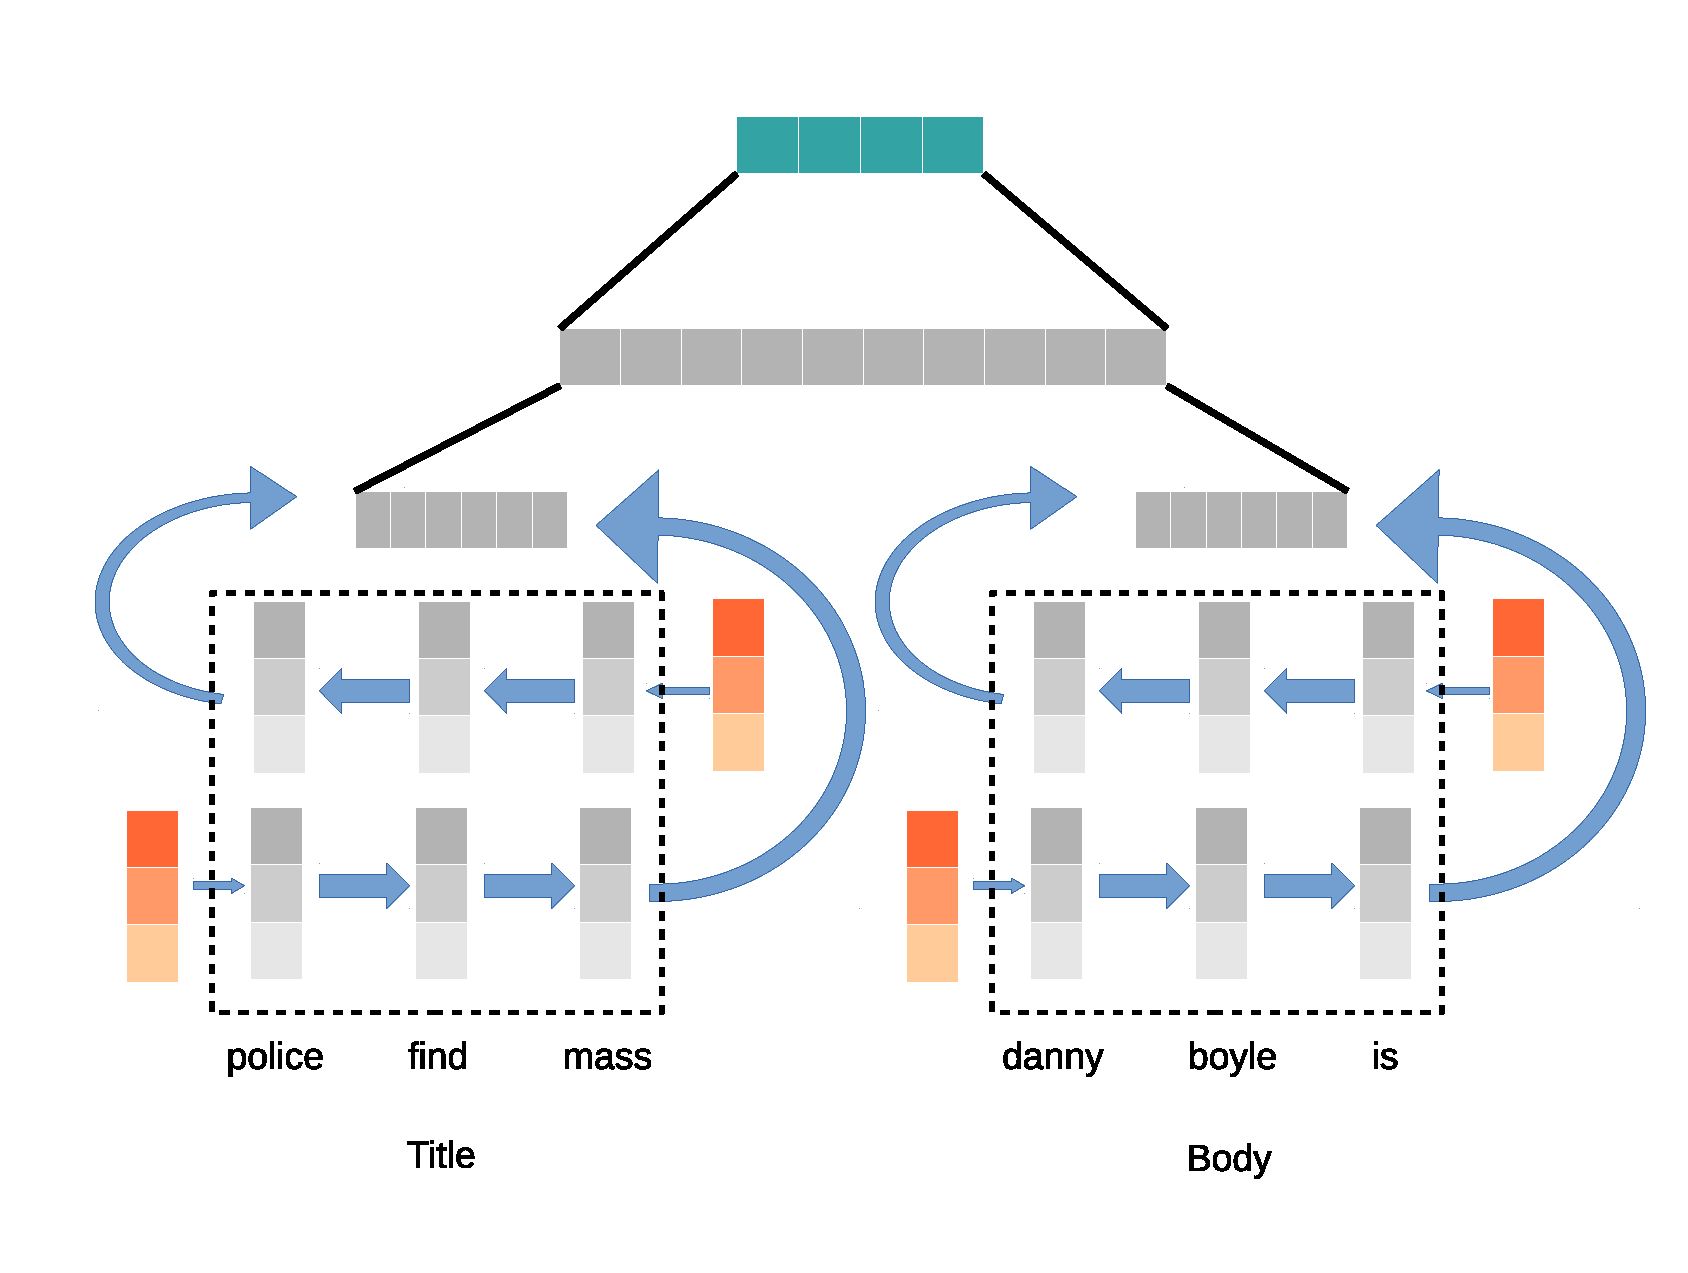
\includegraphics[width=0.8\textwidth]{birnn.eps}
		\caption{Unconditional Bidirectional RNN模型示意图}
		\label{birnn}
	\end{figure}
	\begin{figure}[H]
		\centering
		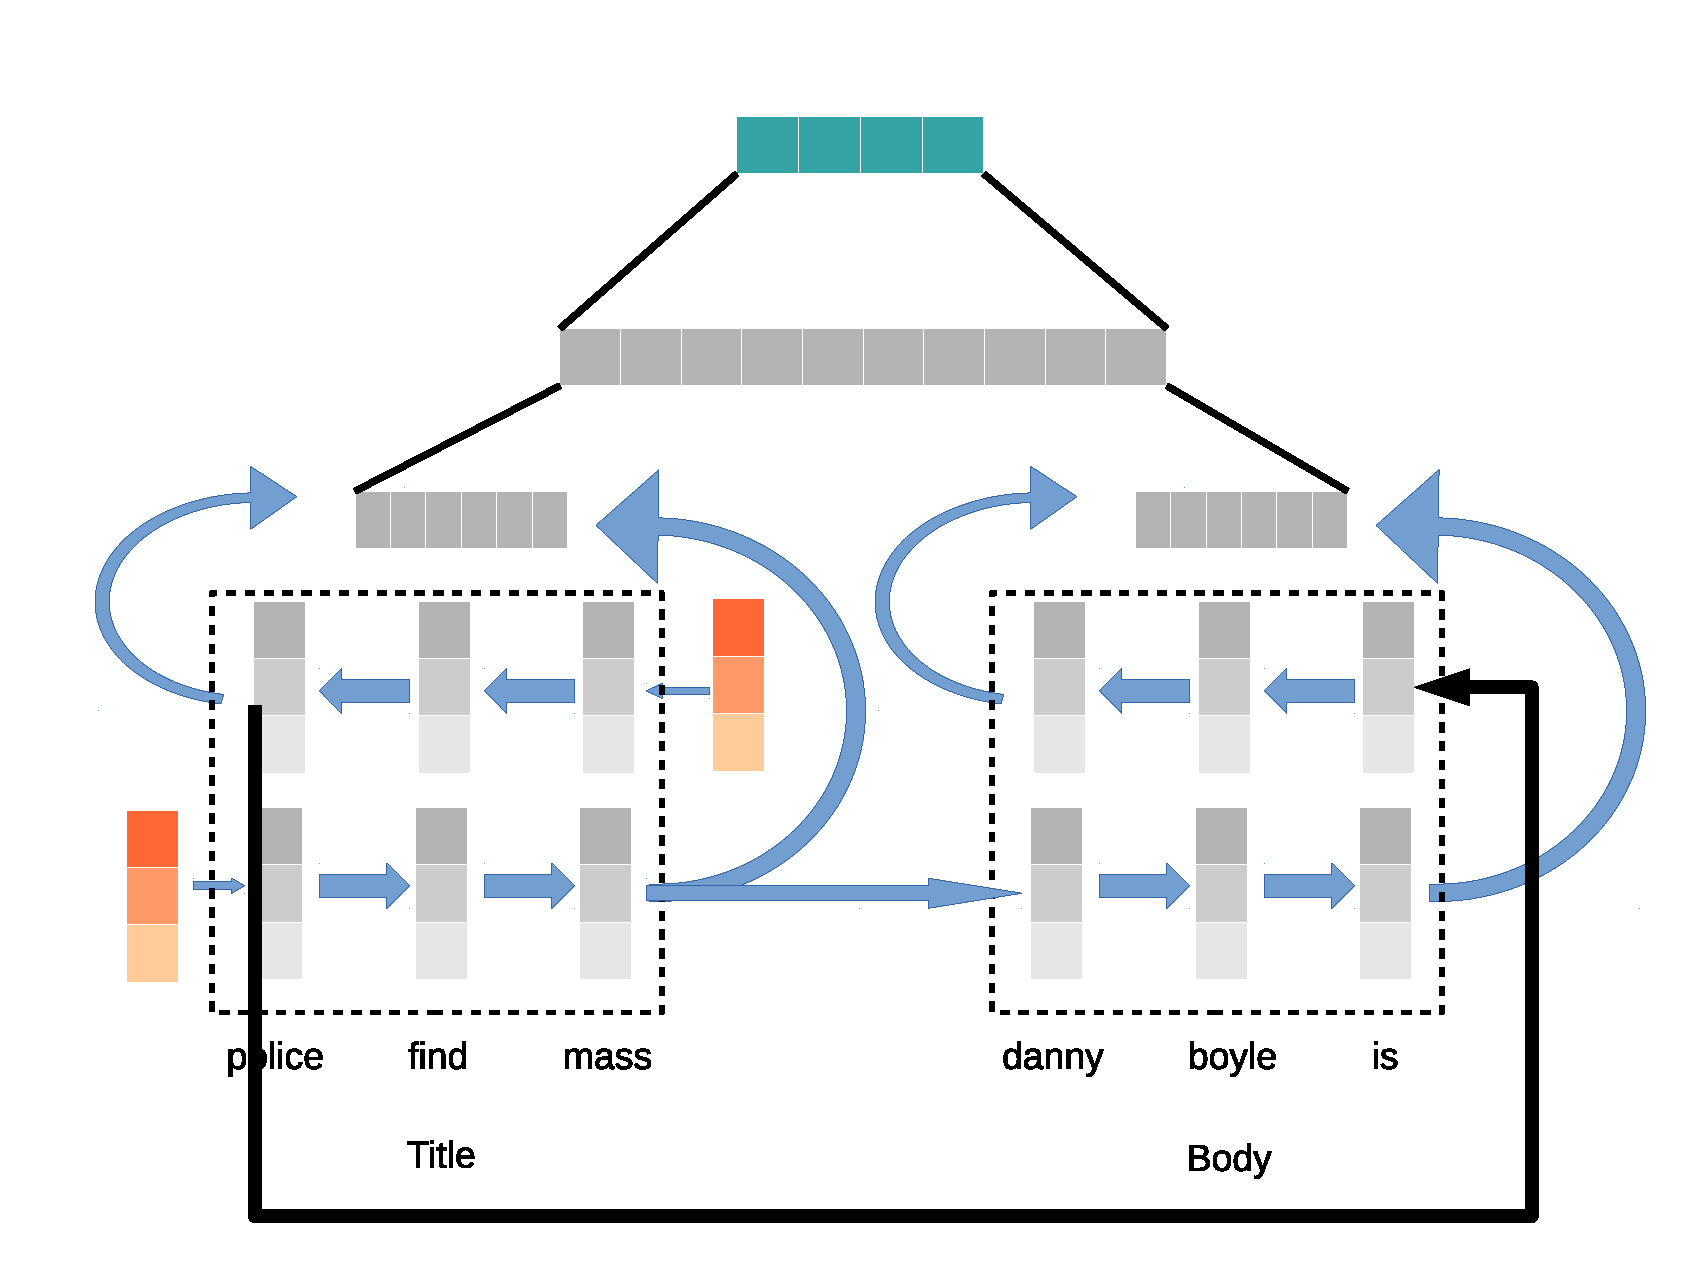
\includegraphics[width=0.8\textwidth]{birnn_cond.eps}
		\caption{Conditional Bidirectional RNN模型示意图}
		\label{birnn_cond}
	\end{figure}
	双向RNN模型将输入序列分别按照顺序和反序输入, 2种顺序得到的最终向量拼接后作为RNN的输出向量. 将标题文本和正文文本的RNN输出向量拼接后送入分类网络进行分类.\\\\
	根据处理正文文本的RNN使用的初始向量的种类, 可以构造2种不同的双向RNN模型:
	\begin{itemize}
		\item Unconditional Bidirectional RNN: 处理正文的RNN使用零向量作为初始向量.
		\item Conditional Bidirectional RNN: 处理正文的RNN使用处理标题的RNN的输出向量作为初始向量. 这种做法在标题和正文之间建立了联系, 可能会取得更好的效果.
	\end{itemize}
	\subsubsection{引入了attention机制的RNN模型}
	\begin{figure}[H]
		\centering
		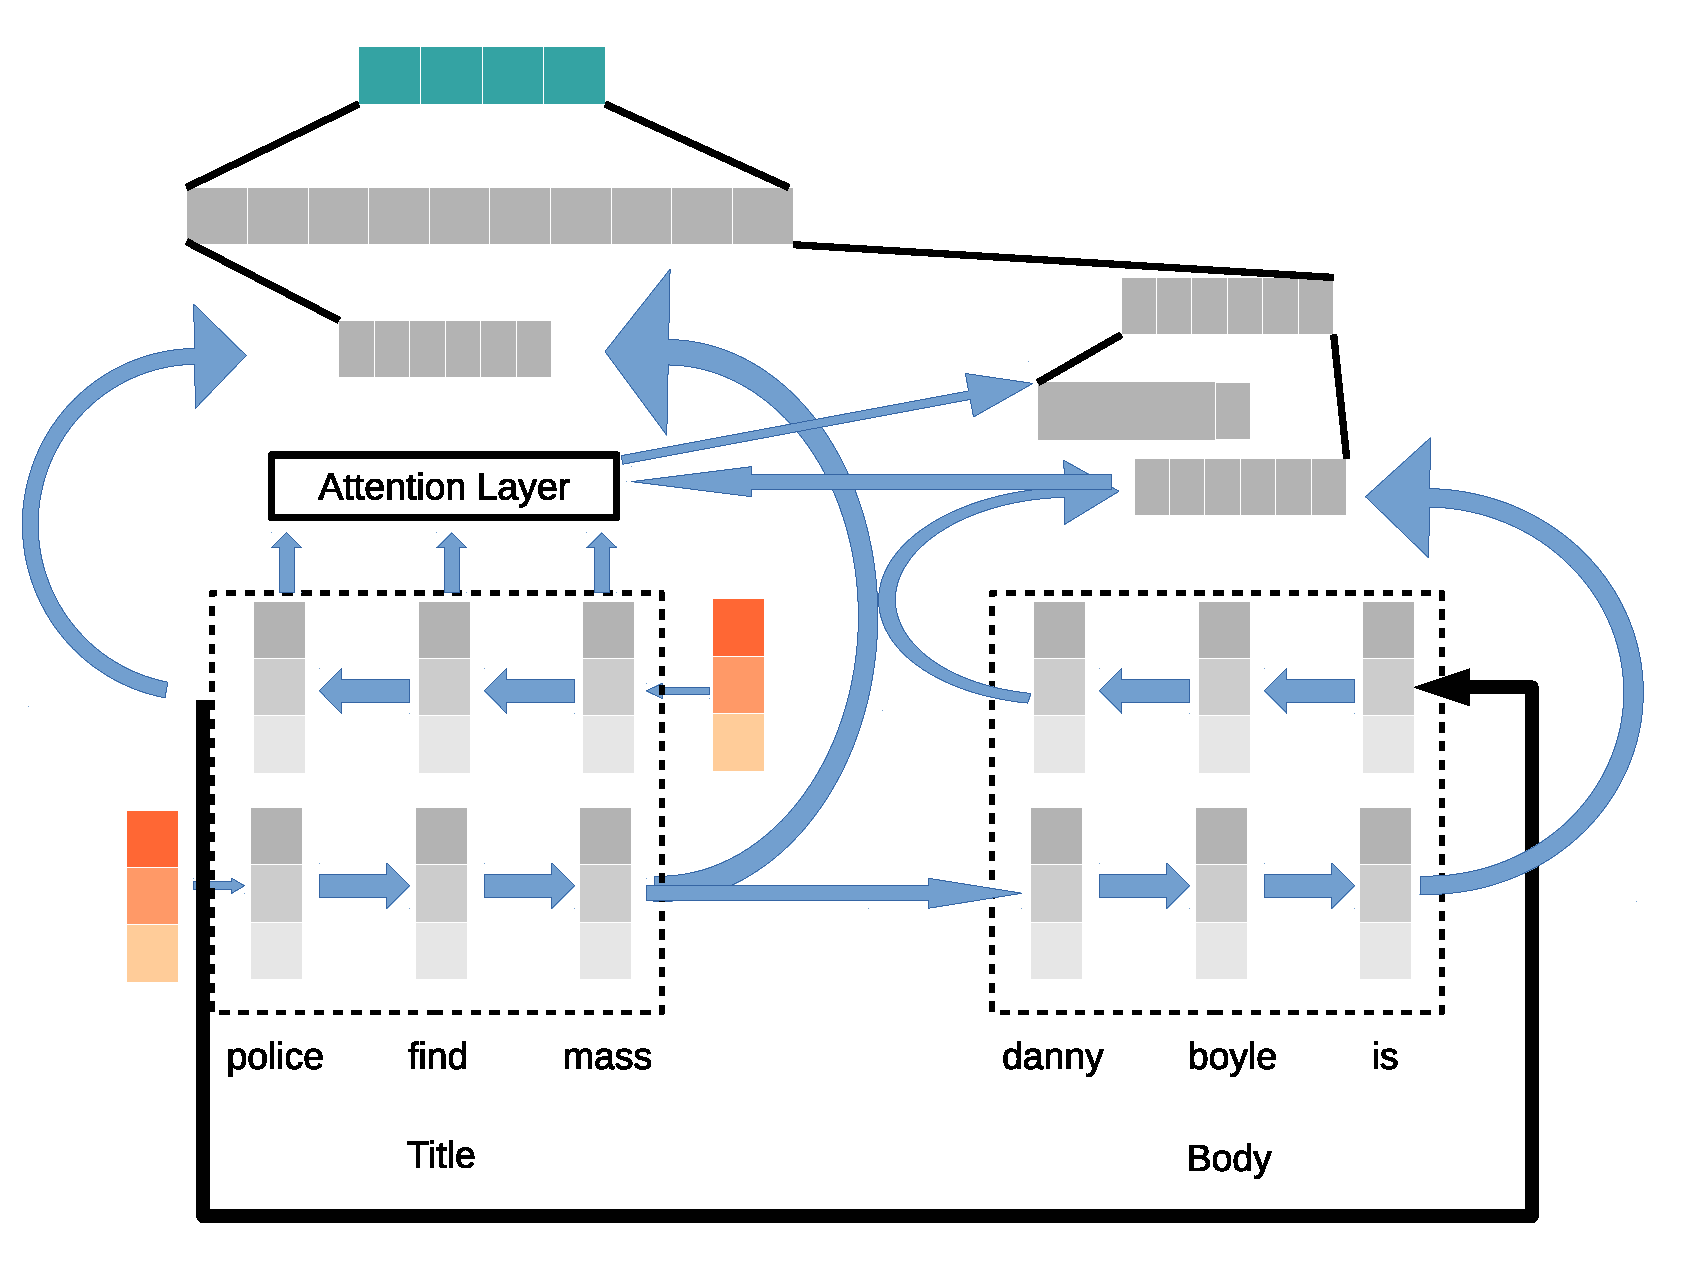
\includegraphics[width=0.8\textwidth]{att1.eps}
		\caption{引入attention的Conditional Bidirectional RNN模型1示意图}
		\label{att1}
	\end{figure}
	\begin{figure}[H]
		\centering
		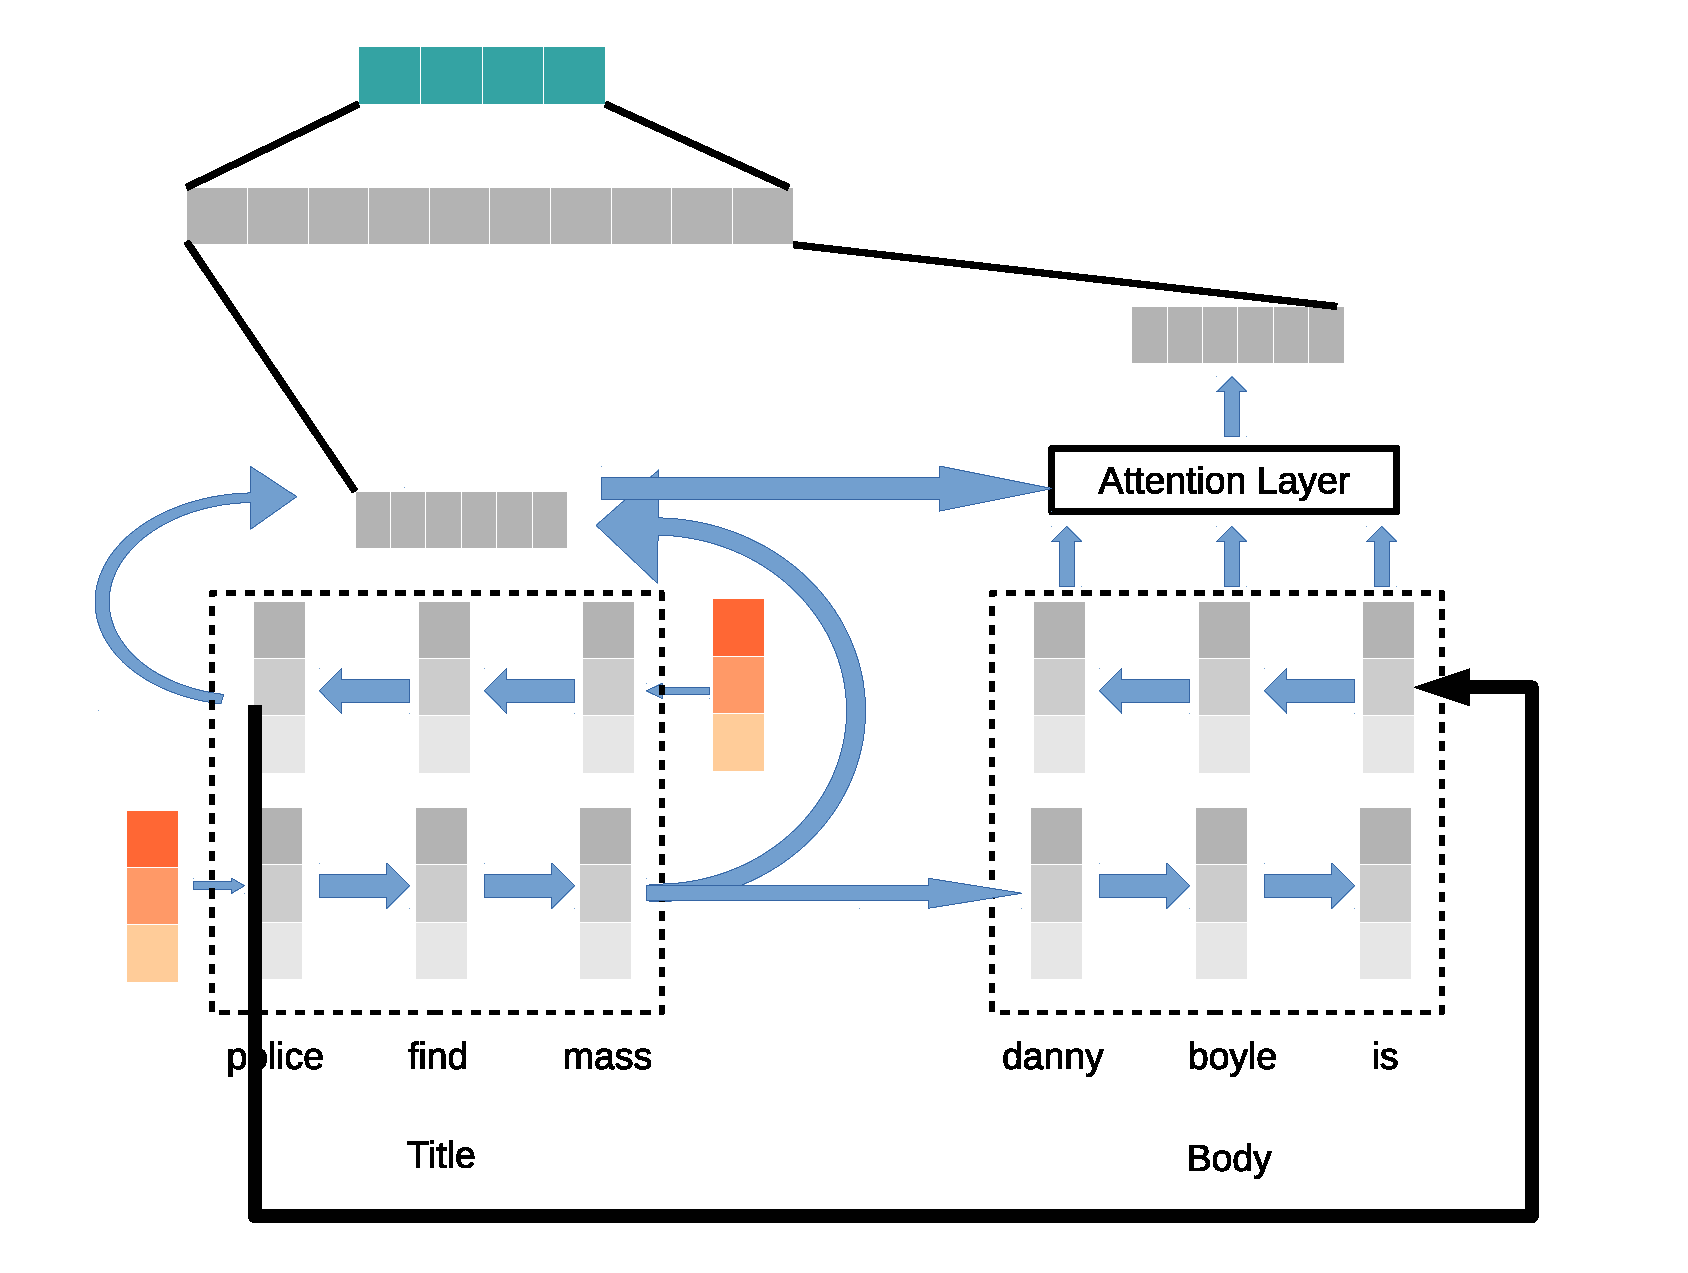
\includegraphics[width=0.8\textwidth]{att2.eps}
		\caption{引入attention的Conditional Bidirectional RNN模型2示意图}
		\label{att2}
	\end{figure}
	在RNN模型的基础上存在许多变种, 其中一种引入了所谓的attention机制\cite{luong2015effective}. Attention机制的原理是根据RNN最后一个单元的输出向量为所有单元的输出向量赋予不同的权重, 各个单元输出向量加权后与最后一个单元的输出向量拼接, 经过一个非线性层后输出. 根据前人的研究和实验验证, 效果较好的权重计算方式为: 最后一个单元的输出$h_T$与各个单元的输出$h_t$做双线性变换$h_T^TWh_t+b$的结果经过softmax函数处理后作为$h_t$的权重, 非线性层的函数可选为$\tanh$.\\\\
	具体到本实验的问题, 由于标题和正文在2个RNN中处理, 可以使用正文RNN的输出向量与标题RNN的所有输出向量做attention, 结果与标题RNN最后的输出向量拼接后进入分类网络.\\\\
	文献\cite{chen2016thorough}对attention模型进行了一定简化, 主要区别是取消了非线性层, 直接使用加权后的结果作为输出向量. 该简化模型同样经修改应用到了本实验中.
	
	\subsection{混合模型}
	\begin{figure}[H]
		\centering
		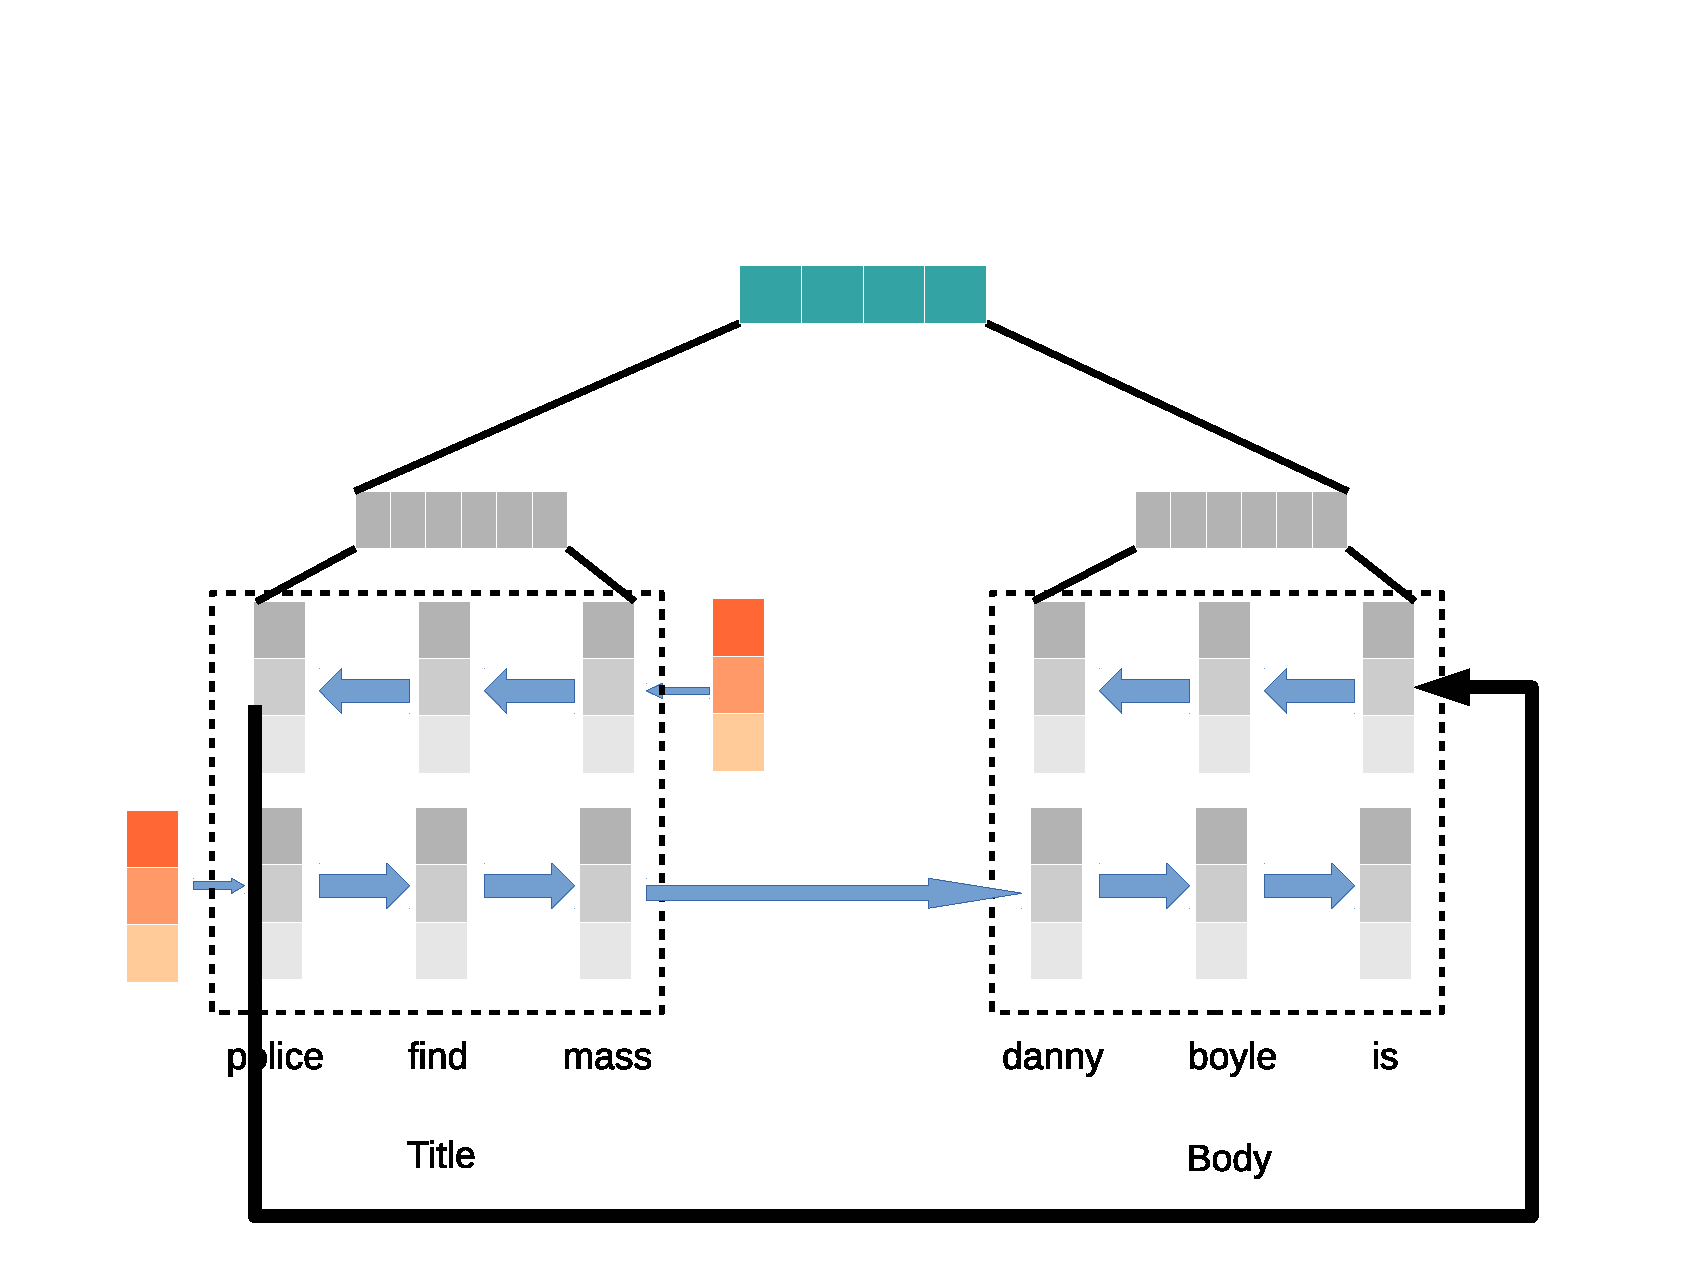
\includegraphics[width=0.8\textwidth]{rcnn.eps}
		\caption{CNN-RNN混合模型示意图}
		\label{rcnn}
	\end{figure}
	混合模型结合了RNN与CNN的pooling操作\cite{lai2015recurrent}, 使用RNN替代CNN中的卷积部分, 在文本分类等任务中有较好的效果. 具体组成如下:
	\begin{itemize}
		\item 卷积层: 使用bidirectional rnn各阶段的输出作为"卷积"结果.
		\item 非线性层: 各阶段的输出经过同一个线性层后被激活函数tanh处理.
		\item 池化层: 对各阶段的输出沿阶段数所在轴做maxpooling.
		\item 分类层: 标题和正文分别经前述3层处理后的输出拼接后经过线性层和softmax得到分类结果.
	\end{itemize}
	
	\section{实验}
	\subsection{实验数据}
	实验数据由Fake News Challenge的主办方提供, 规模在50k篇文章左右, 包含以下2个文件:
	\begin{itemize}
		\item train\_bodies.csv: 正文和对应的ID;
		\item train\_stances.csv: 态度, 标题, 标题对应的正文ID.
	\end{itemize}
	实验中将80\%的数据作为训练集, 20\%的数据作为测试集. 对于Baseline方法, 选择训练集的10\%作为验证集进行10-fold交叉验证; 对于神经网络模型, 由于运行一次耗时较长且数据量有限, 故直接使用全部训练集数据进行网络训练.\\\\
	经过简单分析可以发现提供的数据非常不平衡, 高达73.13\%的例子属于unrelated, 而discuss, agree, disagree的样例仅占17.83\%, 7.36\%和1.68\%. 若直接使用会使得分类结果出现严重偏差, 分类器很容易将所有样例判断为unrelated.\\\\
	常用的处理不平衡数据的方法包括over sampling, under sampling和人为增大损失函数中占比较低的类别的权重. Over sampling对所有占比非最大的种类的数据进行有放回抽样, 直到所有类别的样例数目相等; under sampling则对所有占比非最小的种类的数据进行不放回抽样, 使得所有类别的样例数目相等; 对于某些分类问题常用的损失函数(例如cross entropy函数), 可以人为调整不同类别的权重. 显然实验中使用under sampling得到的数据集规模过小, 不利于深度学习方法的处理, 而调整权重的方法不能解决SGD类优化方法划分batch时很可能出现的某一占比极少的类别在某一个batch中完全不出现的情况从而造成优化速度下降, 因此使用over sampling预处理数据. 需要注意的是over sampling必须在划分训练集和测试集之后在训练集上进行, 否则测试集类别分布的信息会"泄露"到训练集中, 使得模型在测试集上的表现偏好.\\\\
	数据的另一个问题是标题长度和正文长度相差极大, 标题的最大长度<50, 而正文的最大长度>2000, 人类在判断标题与正文的关系时往往阅读正文的开头部分即可, 因此过长的正文对于神经网络模型正确分类很可能意义不大. 出于加速训练和节省内存的考虑, 使用神经网络模型时仅使用正文的开头部分, 为了验证假设, 实验比较了截取不同长度正文时的分类效果.
	\subsection{评价标准}
	实验问题属于多分类问题, 采用以下的评价标准:
	\begin{itemize}
		\item 精确度(accuracy): $\dfrac{\text{被正确分类的样例数}}{\text{样例总数}}$.
		%\item 混淆矩阵(confusion matrix): 矩阵的每一列代表一个类的实例预测, 而每一行表示一个实际的类的实例, 矩阵元素代表该类中样例的数量.
		\item 比赛方的评价方法: 对于每个样例, 若被成功区分related(包括除了unrelated之外的3类)/unrelated, 可得到0.25分, 若被分类正确且属于除了unrelated之外的3类, 则可继续得到0.75分.
		\begin{figure}[H]
			\centering
			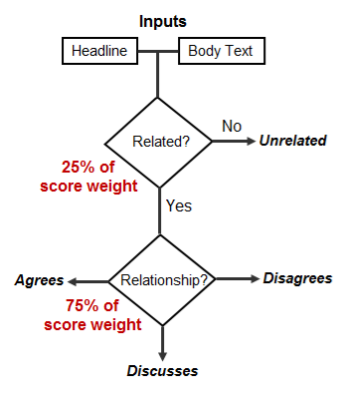
\includegraphics[width=0.5\textwidth]{fnc-eval.png}
			\caption{Fake News Challenge 评分标准}
			\label{fnc-eval}
		\end{figure}
		\item 将多分类问题看做多个二分类问题的组合, 考察模型在每个二分类问题上的表现, 包括precision, recall和F1-score.
	\end{itemize}
	\subsection{模型实现, 参数设置与运行环境}
	Baseline模型由比赛主办方提供, 基于scikit-learn中的GBDT分类器实现. 其余的神经网络模型基于PyTorch框架\footnote{http://pytorch.org/}实现. PyTorch框架提供了常见的CNN, RNN单元, 同时提供了自动求导功能, GPU加速功能和多种优化器, 便于使用者搭建灵活的网络结构和使用GPU加速训练.\\\\
	参数设置见附录, 本实验无意探究众多模型超参数对结果的影响, 因此仅比较了少数超参数的不同和模型结构的不同对分类结果的影响.\\\\
	Baseline模型运行平台硬件配置为Intel i7-6600u@3.0GHz, 16GB RAM, 软件配置为Ubuntu 16.04 LTS Desktop, Python 3.6.0. 神经网络模型运行平台为Amazon Web Services的p2.xlarge实例, 硬件配置为4核心CPU, 64GB RAM, Nvidia K80 GPU(显存12GB)x1, 软件配置为Ubuntu 16.04 LTS Server, Python 3.6.0.
	\subsection{实验结果}
	\subsubsection{词向量维度的影响}
	\begin{figure}[H]
		\centering
		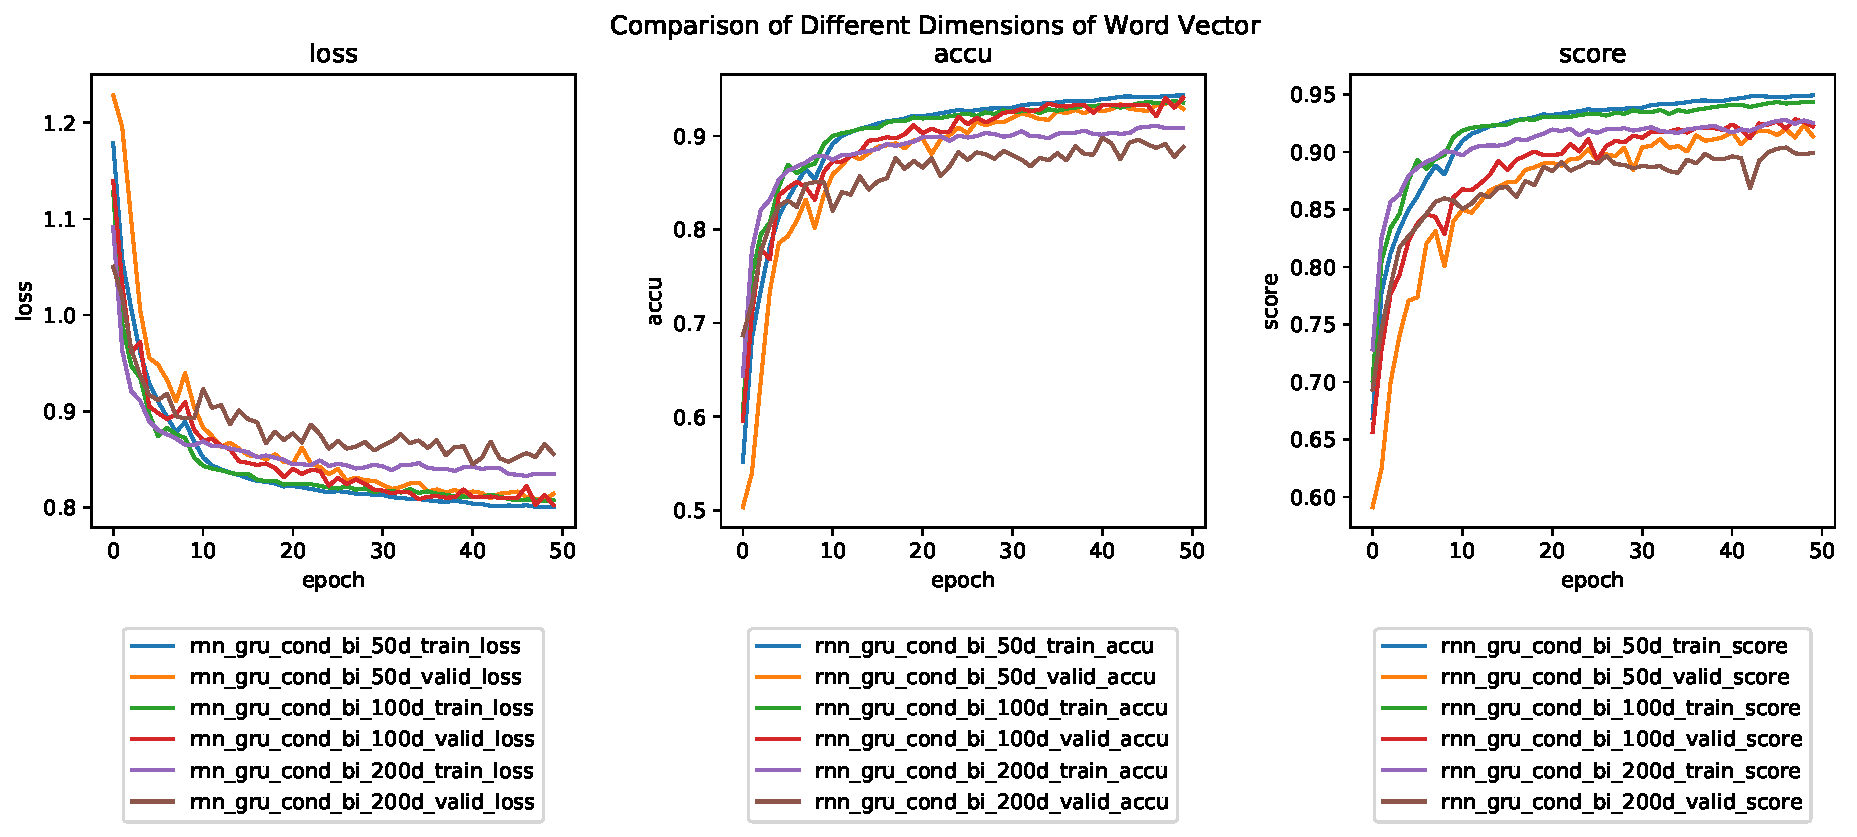
\includegraphics[width=\textwidth]{comparison_of_different_dimensions_of_word_vector.pdf}
		\caption{不同词向量维度下的结果比较}
		\label{comparison_of_different_dimensions_of_word_vector}
	\end{figure}
	\begin{table}[H]
		\centering
		\caption{不同词向量维数在测试集上的最好表现}
		\label{dimperf}
		\begin{tabular}{@{}ccc@{}}
			\toprule
			\textbf{Dim of Word Vector}                  & \textbf{Accuracy} & \textbf{Score}  \\ \midrule
			50   & 0.9356            & 0.9235          \\
			100                 & \textbf{0.9406}            & \textbf{0.9285}          \\
			200                & 0.8872            & 0.9040          \\ \bottomrule
		\end{tabular}
	\end{table}
	GLoVe模型提供了多种维度的词向量. 词向量维数过低会导致词间关系无法充分体现, 词向量维数过高则会大幅增加模型参数数量, 容易出现过拟合, 同时训练速度下降. 实验中分别选取了长度为50, 100和200的词向量, 比较它们在Conditional Bidirectional RNN模型上的效果. 可以发现长度为50和100的词向量表现相近, 且均好于长度为200的词向量. 原因可能是用于训练的数据量不大, 高维词向量更强的表现力难以在小规模数据集上体现, 反而因难以优化导致表现不好.\\\\ 出于提高训练速度的考虑, 后续实验均选择50维的词向量.
	\subsubsection{词向量训练方式的影响}
	\begin{figure}[H]
		\centering
		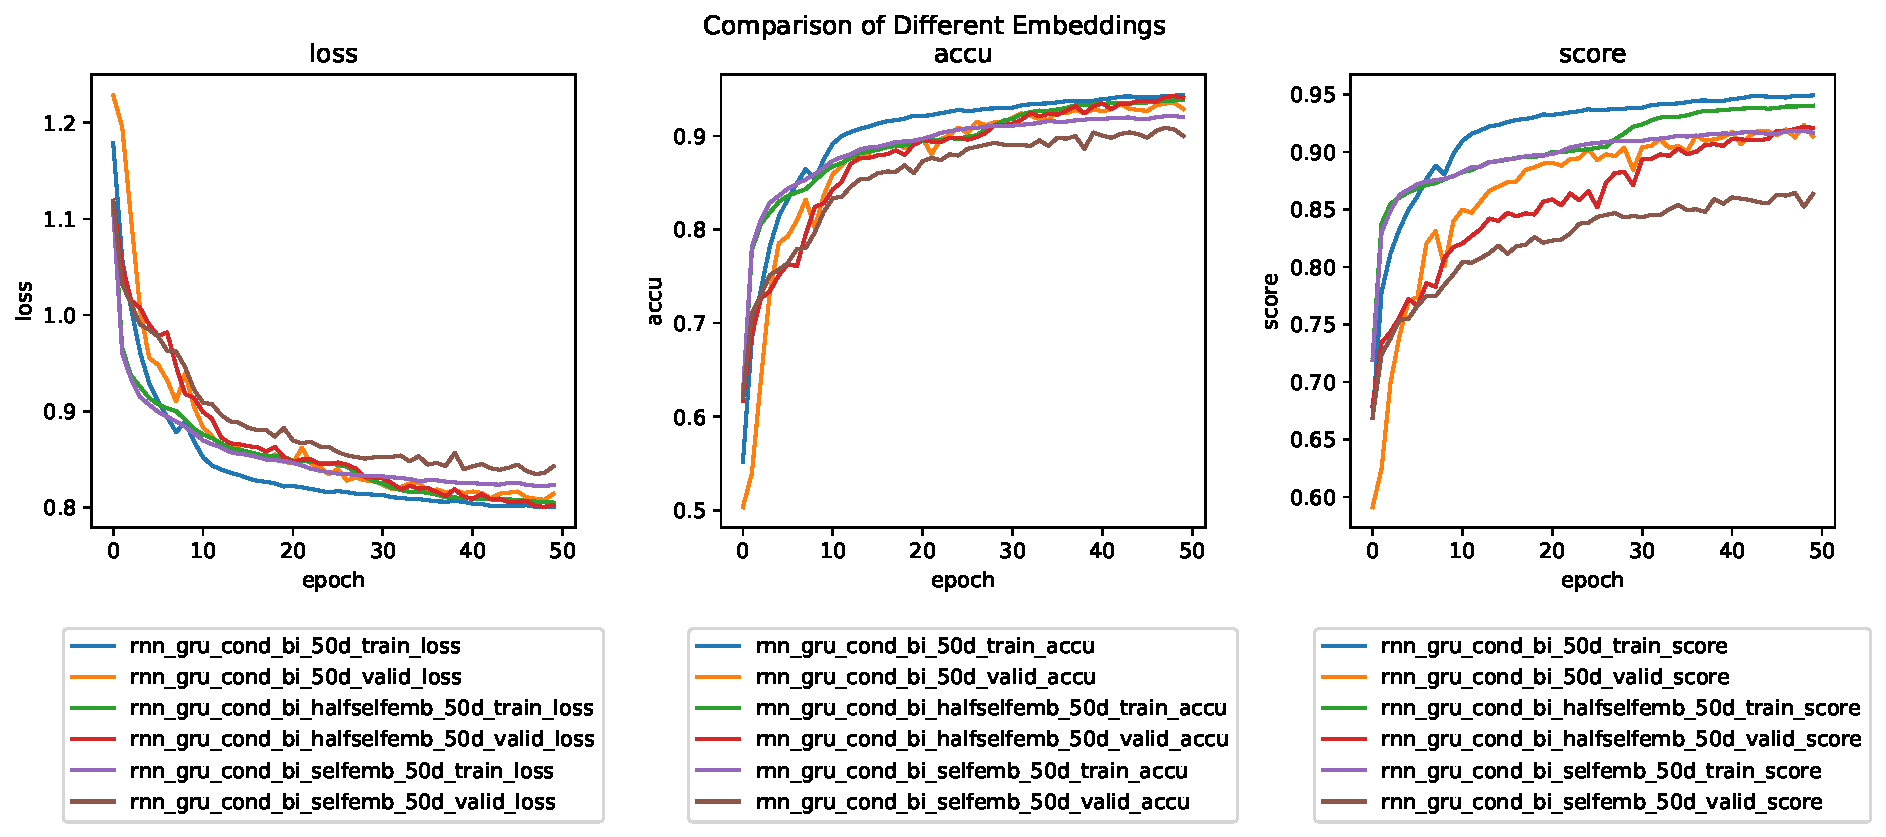
\includegraphics[width=\textwidth]{comparison_of_different_embeddings.pdf}
		\caption{不同词向量训练方式的结果比较}
		\label{comparison_of_different_embeddings}
	\end{figure}
	\begin{table}[H]
		\centering
		\caption{不同词向量训练方式在测试集上的最好表现}
		\label{embperf}
		\begin{tabular}{@{}ccc@{}}
			\toprule
			\textbf{Embedding}                  & \textbf{Accuracy} & \textbf{Score}  \\ \midrule
			GLoVe Fixed   & 0.9356            & \textbf{0.9235}          \\
			GLoVe Not Fixed                 & \textbf{0.9426}            & 0.9219          \\
			Self Embedding                & 0.9087 & 0.8645          \\ \bottomrule
		\end{tabular}
	\end{table}
	本实验比较了3种词向量的训练方式: 直接使用预训练的模型(GLoVe Fixed), 在预训练模型基础上调整(GLoVe Not Fixed)以及从零开始训练(Self Embedding). 由结果可见直接使用预训练模型效果较好, 在预训练模型基础上调整词向量对结果没有改善, 而从零开始训练词向量的结果最差. 原因是用于训练的文本量太小, 无法正确反应词汇之间的关系.
	\subsubsection{正文截取长度的影响}
	\begin{figure}[H]
		\centering
		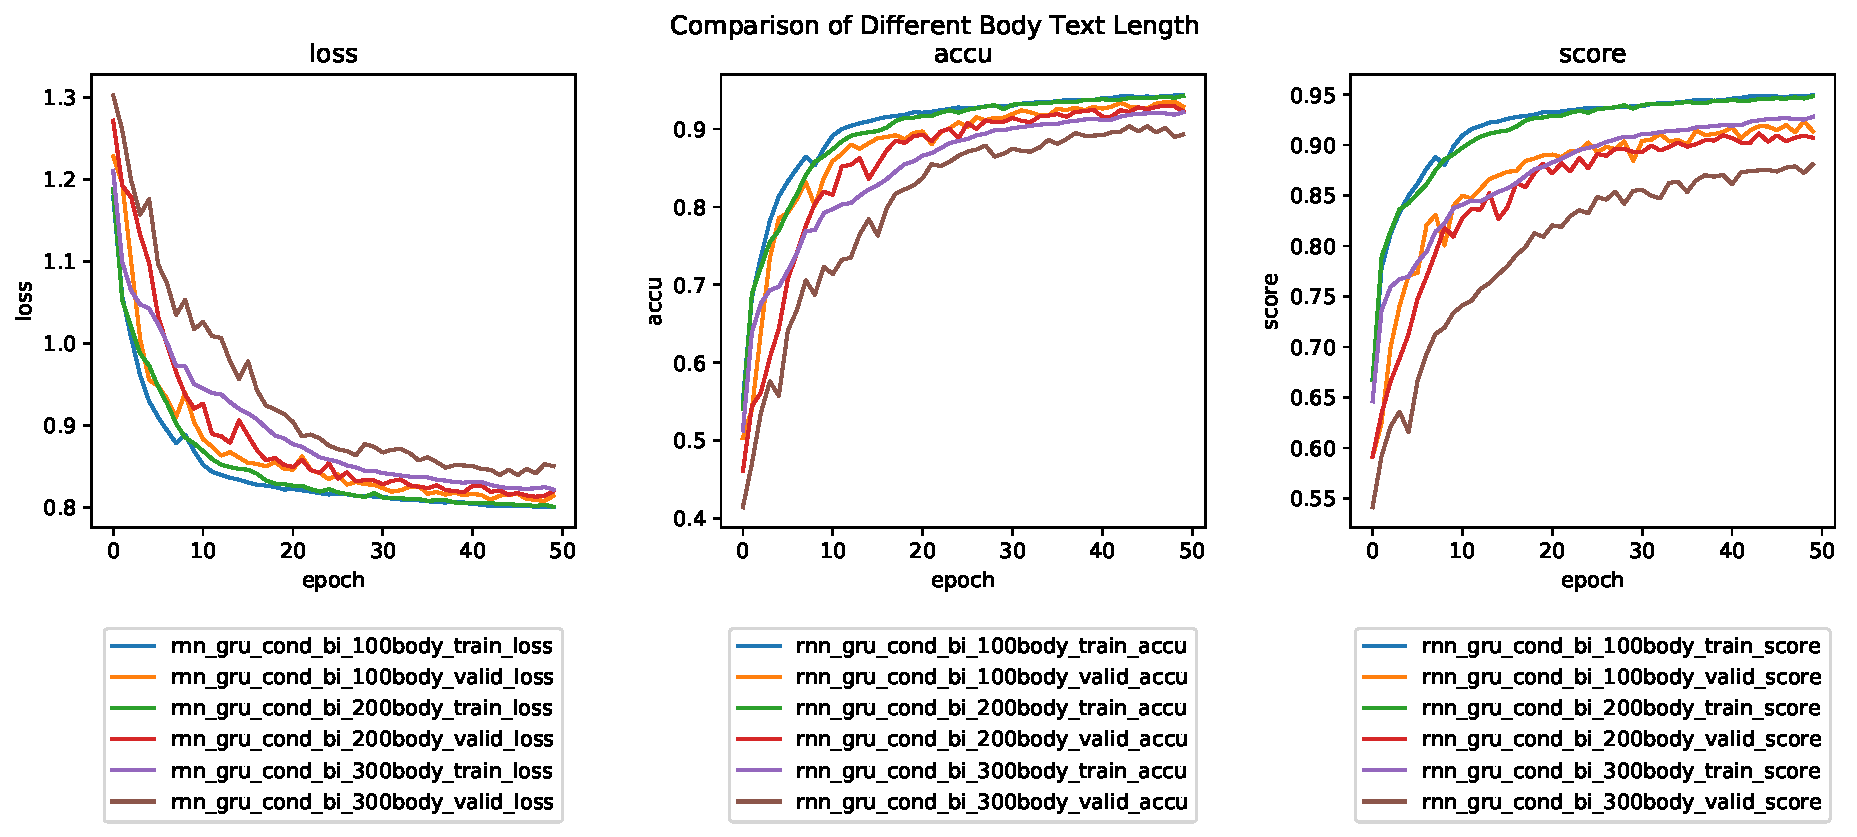
\includegraphics[width=\textwidth]{comparison_of_different_body_text_length.pdf}
		\caption{不同正文截取长度下的结果比较}
		\label{comparison_of_different_body_text_length}
	\end{figure}
	\begin{table}[H]
		\centering
		\caption{不同正文截取长度在测试集上的最好表现}
		\label{lenperf}
		\begin{tabular}{@{}ccc@{}}
			\toprule
			\textbf{Body Text Length}                  & \textbf{Accuracy} & \textbf{Score}  \\ \midrule
			100   & \textbf{0.9356}            & \textbf{0.9235}          \\
			200                 & 0.9220            & 0.9116          \\
			300                & 0.8930 & 0.8811          \\ \bottomrule
		\end{tabular}
	\end{table}
	正文截取长度过短可能导致正文的态度无法被充分提取, 截取长度过长则会大幅增加模型的资源消耗和训练时间. 实验比较了正文截取长度分别为100, 200和300时Conditional Bidirectional RNN模型的表现. 可以发现截取长度为100和200时模型表现相近, 且均好于截取长度为300时的表现. 原因可能是过长的正文使得模型更难训练, 同时正文与标题长度差距过大会减弱模型对标题特征的提取能力.\\\\
	出于提高训练速度的考虑, 后续实验均选择100的正文截取长度.
	\subsubsection{RNN单元种类的影响}
	\begin{figure}[H]
		\centering
		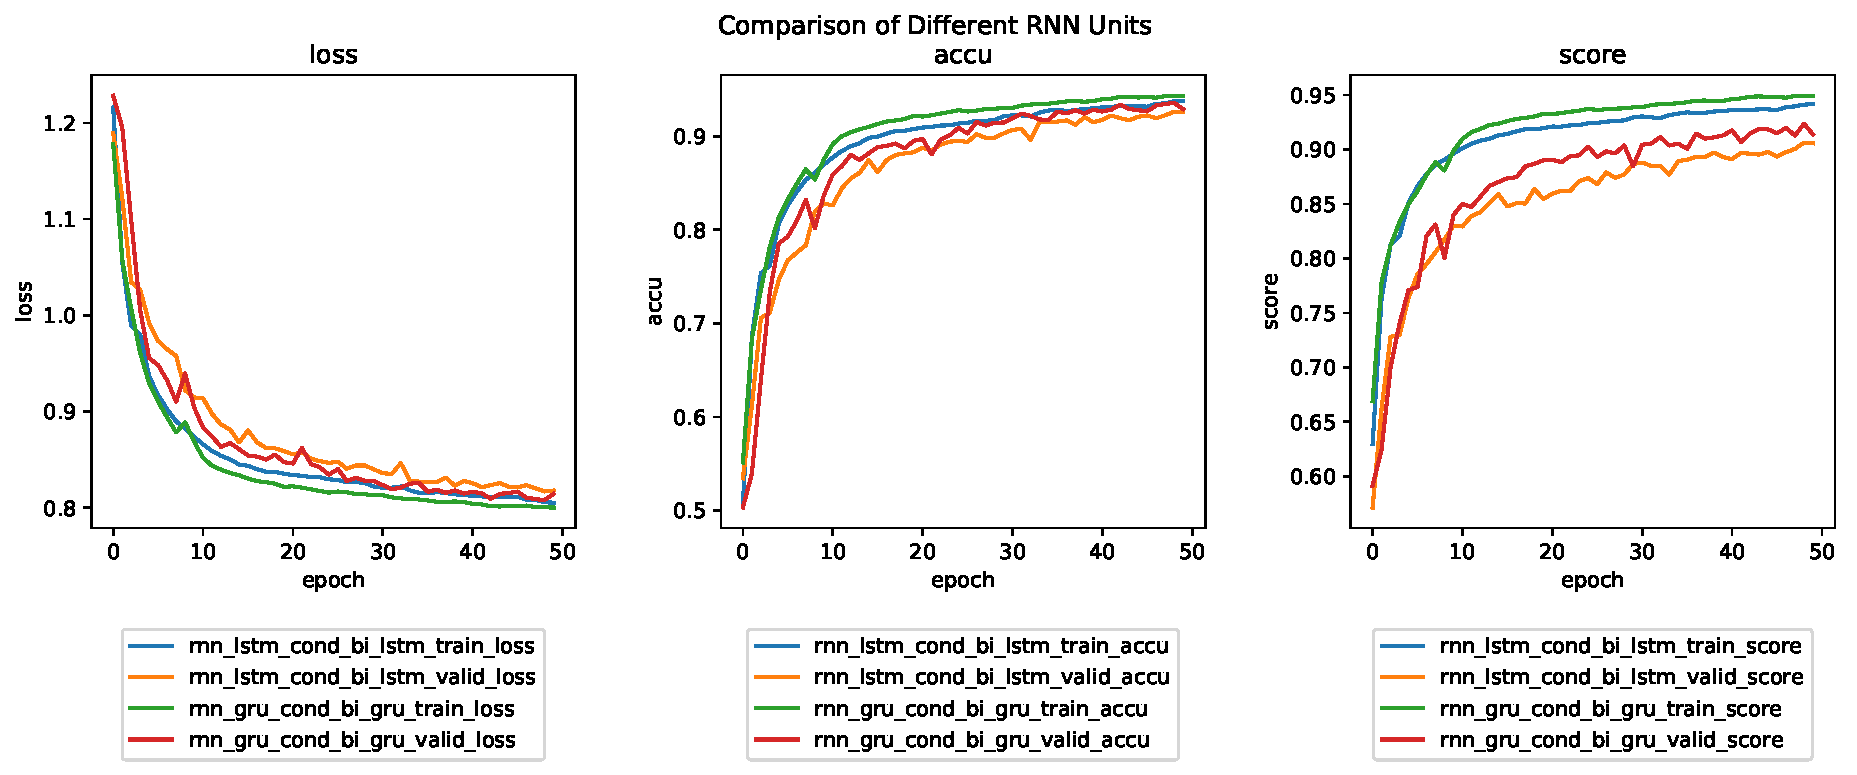
\includegraphics[width=\textwidth]{comparison_of_different_rnn_units.pdf}
		\caption{不同RNN单元的结果比较}
		\label{comparison_of_different_rnn_units}
	\end{figure}
	\begin{table}[H]
		\centering
		\caption{不同RNN单元在测试集上的最好表现}
		\label{rnnunitperf}
		\begin{tabular}{@{}ccc@{}}
			\toprule
			\textbf{Type of RNN}                  & \textbf{Accuracy} & \textbf{Score}  \\ \midrule
			GRU   & \textbf{0.9356}            & \textbf{0.9235}          \\
			LSTM                 & 0.9263            & 0.9063          \\ \bottomrule
		\end{tabular}
	\end{table}
	两种RNN单元在测试集上的表现非常接近, 鉴于GRU的训练速度略快一些, 后续实验均选用GRU作为RNN单元.
	\subsubsection{模型效果比较}
	\begin{figure}[H]
		\centering
		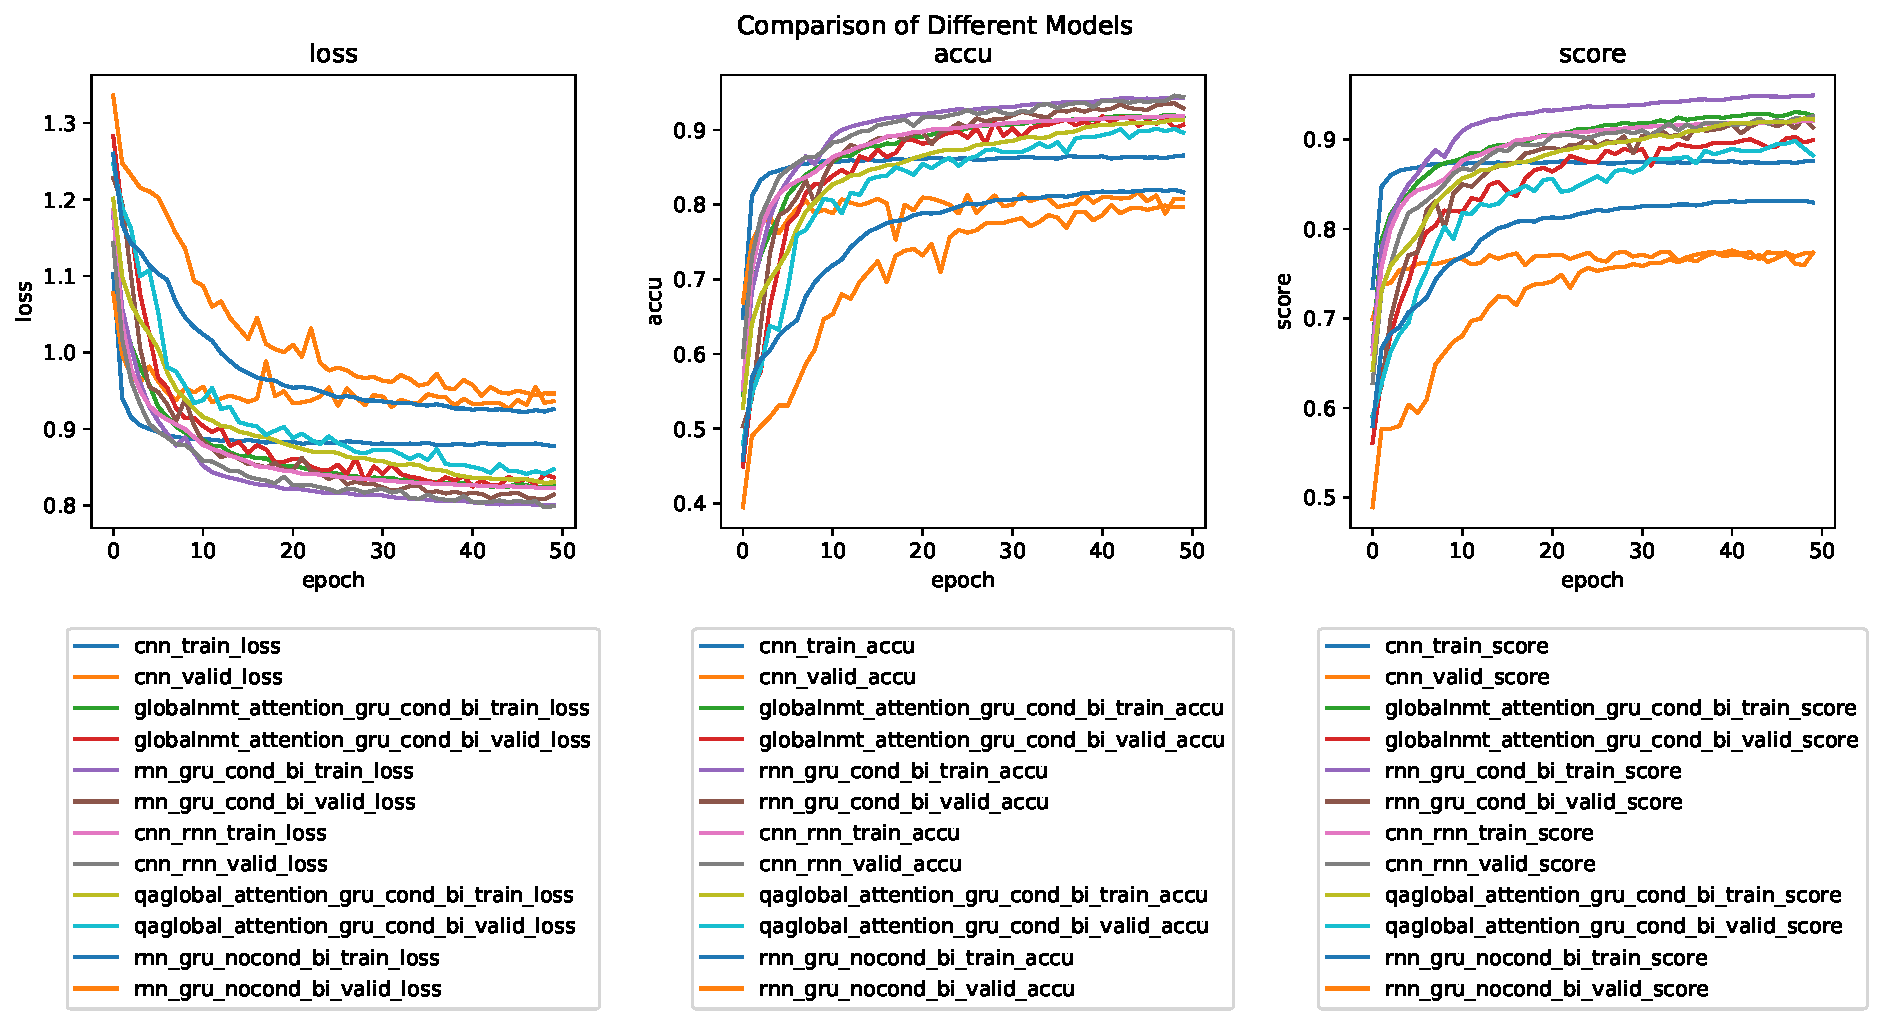
\includegraphics[width=\textwidth]{comparison_of_different_models.pdf}
		\caption{不同模型的结果比较}
		\label{comparison_of_different_models}
	\end{figure}

	\begin{table}[H]
		\centering
		\caption{不同模型在测试集上的最好表现}
		\label{performance}
		\begin{tabular}{@{}ccccc@{}}
			\toprule
			\multirow{2}{*}{\textbf{Model}} & \multicolumn{2}{c}{\textbf{Train}} & \multicolumn{2}{c}{\textbf{Test}} \\ \cmidrule(l){2-5} 
			& \textbf{Accuracy}       & \textbf{Score}      & \textbf{Accuracy}      & \textbf{Score} \\ \cmidrule(l){1-5}
			Baseline & - & - & 0.8774 & 0.7953 \\
			CNN & 0.8613 & 0.8741 & 0.8122 & 0.7747 \\
			Unconditional Bidirectional RNN & 0.8175&0.8311 &0.7860 &0.7760 \\
			Conditional Bidirectional RNN &0.9431 &0.9486 &0.9356 &0.9235 \\
			Attention RNN I &0.9200 &0.9308 &0.9156 &0.9030 \\
			Attention RNN II &0.9112 &0.9211 &0.8982 &0.8986 \\
			CNN-RNN &0.9188 &0.9203 &\textbf{0.9438} &\textbf{0.9262} \\
			\bottomrule
		\end{tabular}
	\end{table}

	\begin{table}[H]
	\centering
	\caption{Agree分类结果}
	\label{agree}
	\begin{tabular}{@{}ccccccc@{}}
		\toprule
		\multirow{2}{*}{\textbf{Model}} & \multicolumn{3}{c}{\textbf{Train}} & \multicolumn{3}{c}{\textbf{Test}} \\ \cmidrule(l){2-7} 
		& \textbf{Precision}       & \textbf{Recall}      & \textbf{F1}      & \textbf{Precision}      & \textbf{Recall}      & \textbf{F1}      \\ \cmidrule(l){1-7}
		Baseline & - & - & - &0.6051 & 0.1549 & 0.2466 \\
		CNN&0.8946&0.8654&0.8797&0.4887&0.7203&0.5823\\
		Unconditional Bidirectional RNN&0.8569&0.8143&0.8351&0.4718&0.6913&0.5608\\
		Conditional Bidirectional RNN&0.9361&0.9186&0.9273&0.7507&0.829&0.7879\\
		Attention RNN I&0.8865&0.9136&0.8999&0.5902&0.8391&0.693\\
		Attention RNN II&0.8657&0.9406&0.9016&0.6181&\textbf{0.8609}&0.7196\\
		CNN-RNN&0.9216&0.9048&0.9131&\textbf{0.8211}&0.7783&\textbf{0.7991}\\
		\bottomrule
	\end{tabular}
	\end{table}
	\begin{table}[H]
		\centering
		\caption{Disagree分类结果}
		\label{disagree}
		\begin{tabular}{@{}ccccccc@{}}
			\toprule
			\multirow{2}{*}{\textbf{Model}} & \multicolumn{3}{c}{\textbf{Train}} & \multicolumn{3}{c}{\textbf{Test}} \\ \cmidrule(l){2-7} 
			& \textbf{Precision}       & \textbf{Recall}      & \textbf{F1}      & \textbf{Precision}      & \textbf{Recall}      & \textbf{F1}      \\ \cmidrule(l){1-7}
			Baseline & -& -& -&0.25 & 0.0185 & 0.0345 \\
			CNN&0.9186&0.9677&0.9425&0.4595&0.7553&0.5714\\
			Unconditional Bidirectional RNN&0.9141&0.8065&0.857&0.3746&0.6596&0.4778\\
			Conditional Bidirectional RNN&0.95&0.9188&0.9342&\textbf{0.6857}&\textbf{0.766}&\textbf{0.7236}\\
			Attention RNN I&0.9412&0.8598&0.8987&0.6536&0.6223&0.6376\\
			Attention RNN II&0.9691&0.8113&0.8832&0.6269&0.6702&0.6478\\
			CNN-RNN&0.9343&0.8032&0.8638&0.6413&0.6277&0.6344\\
			\bottomrule
		\end{tabular}
	\end{table}
	\begin{table}[H]
		\centering
		\caption{Discuss分类结果}
		\label{discuss}
		\begin{tabular}{@{}ccccccc@{}}
			\toprule
			\multirow{2}{*}{\textbf{Model}} & \multicolumn{3}{c}{\textbf{Train}} & \multicolumn{3}{c}{\textbf{Test}} \\ \cmidrule(l){2-7} 
			& \textbf{Precision}       & \textbf{Recall}      & \textbf{F1}      & \textbf{Precision}      & \textbf{Recall}      & \textbf{F1}      \\ \cmidrule(l){1-7}
			Baseline & -& -& -& 0.6608 & 0.8483 & 0.7429 \\
			CNN&0.8853&0.7601&0.818&0.6859&0.6957&0.6907\\
			Unconditional Bidirectional RNN&0.8057&0.8071&0.8064&0.6551&0.7183&0.6852\\
			Conditional Bidirectional RNN&0.9366&0.968&0.952&0.8644&0.9206&0.8916\\
			Attention RNN I&0.9041&0.9517&0.9273&0.8286&0.8931&0.8596\\
			Attention RNN II&0.9045&0.954&0.9286&0.7937&0.9035&0.8451\\
			CNN-RNN&0.8909&0.9728&0.93&\textbf{0.8725}&\textbf{0.9245}&\textbf{0.8978}\\
			\bottomrule
		\end{tabular}
	\end{table}
	\begin{table}[H]
		\centering
		\caption{Unrelated分类结果}
		\label{unrelated}
		\begin{tabular}{@{}ccccccc@{}}
			\toprule
			\multirow{2}{*}{\textbf{Model}} & \multicolumn{3}{c}{\textbf{Train}} & \multicolumn{3}{c}{\textbf{Test}} \\ \cmidrule(l){2-7} 
			& \textbf{Precision}       & \textbf{Recall}      & \textbf{F1}      & \textbf{Precision}      & \textbf{Recall}      & \textbf{F1}      \\ \cmidrule(l){1-7}
			Baseline & -& -& -& 0.9564 & \textbf{0.9849} & \textbf{0.9704} \\
			CNN&0.7603&0.8521&0.8036&0.9104&0.8513&0.8798\\
			Unconditional Bidirectional RNN&0.7243&0.8443&0.7797&0.9124&0.8325&0.8706\\
			Conditional Bidirectional RNN&0.95&0.9671&0.9585&\textbf{0.9822}&0.9537&0.9678\\
			Attention RNN I&0.9364&0.9394&0.9379&0.9805&0.9237&0.9513\\
			Attention RNN II&0.919&0.9388&0.9288&0.978&0.9063&0.9408\\
			CNN-RNN&0.9182&0.9793&0.9478&0.9747&0.9656&0.9701\\
			\bottomrule
		\end{tabular}
	\end{table}

	实验比较了前述模型在测试集上的效果, 总结如下:\\\\
	Baseline模型虽然在测试集上的整体表现一般, 但在进行related/unrelated分类时效果最好, 原因是Baseline模型中的许多特征是从单词/短语层面直接比较文本的相似程度, 因此能够很好地判断2个文本的相关性. 但Baseline模型中关于态度的特征很少, 故在区别agree/disagree/discuss时表现很差.\\\\
	CNN模型和Unconditional Bidirectional RNN模型的表现较差, 甚至不如Baseline模型, 原因是2个模型中只有对标题文本和正文文本分别处理的部分, 标题和正文之间的联系实际上只能靠最后一层的分类器来提取, 极大地影响了分类效果.\\\\
	Conditional Bidirectional RNN模型通过将处理标题的RNN的输出作为处理正文的RNN的输入, 建立了标题与正文之间的联系, 因此在测试集上取得了较高的精确度.\\\\
	引入Attention机制的RNN模型的表现与常规的RNN相比并没有提高, 甚至有所下降. 观察结果可以发现该模型在预测related关系时在测试集上表现较差, 可能是over sampling造成的影响.\\\\
	CNN-RNN模型在测试集上表现最好. 卷积层的引入使得模型能够充分利用RNN中每一步的信息, 提高了模型对文本特征的抓取能力.\\\\
	分别观察各个模型在4种关系上的分类表现可以发现, 尽管over sampling等方法可以一定程度上避免模型过早收敛, 但原始数据的不平衡对分类仍然造成了较大的影响. 在原始数据中极少的agree, disagree两种类型上分类时, 各个模型在测试集上的表现显著差于训练集; 在稍多一些的dicuss上分类时, 测试集表现与训练集表现的差距会缩小; 在最多的unrelated类型上分类时, 测试集的表现甚至略好于训练集.

	\section{结论}
	本实验尝试在stance detection问题上使用不同的深度学习模型, 其中Conditional Bidirectional RNN模型和CNN-RNN模型都取得了不错的分类效果. 深度学习模型不需要人工提取特征, 也能够在该问题上取得较好的结果, 但缺陷是模型的可解释性较差. 同时也应当注意到基于特征工程的传统方法在特征选取得当时, 同样能够在特定的问题(如unrelated的分类)上取得很好的效果. 无论是特征工程方法还是深度学习模型, 都需要对问题本身有深入的理解才能提取出恰当的特征/构建合理的网络结构, 从而更好地解决问题.
	
	\bibliographystyle{unsrt}
	\renewcommand{\refname}{参考文献}
	\bibliography{final_report_bib}
	\clearpage
	
	\pagenumbering{roman}
	\appendix
	\section{运行参数设置}
	除特殊说明外, 程序使用的运行参数默认如下:
	\begin{table}[H]
		\centering
		\caption{运行默认参数}
		\label{defaultparams}
		\begin{tabular}{@{}ccc@{}}
			\toprule
			\textbf{Parameter}                  & \textbf{Meaning} & \textbf{Default Value}  \\ \midrule
			datapath & 预训练word2vec模型所在文件夹 & "./data"          \\
			word2vecmodelfile & 预训练word2vec模型文件 & "glove.twitter.27B.50d.txt"          \\
			fix\_embedding & 训练过程中不更新词向量 & False          \\
			train\_ratio & 训练集比例 & 0.8          \\
			remove\_stopwords & 是否除去文本中的stopwords & False         \\
			batch\_size & 单个batch大小 & 384          \\
			epoch & 在整个训练集上的迭代次数 & 50 \\ 
			cuda & 是否开启CUDA加速(需要NVIDIA GPU支持) & False\\
			lr & 学习率 & 0.001\\
			weight\_decay & L2罚项系数 & 1e-6\\
			title\_trunc & 标题截取长度 & 40\\
			body\_trunc & 正文截取长度 & 100\\
			seed & 随机数种子 & 0\\
			wechat & 开启微信通知功能, 通过文件传输助手实时发送训练进度 & False\\
			model & 模型名称 & 必填\\
			modelpath & 存储训练中间结果的文件夹 & 必填\\
			optimizer & 优化算法名称 & "Adam"\\
			selfemb & 指定维数时自行训练词向量, 不使用预训练模型 & None\\
			resume & 从modelpath中最后一个checkpoint恢复训练 & False\\
			\bottomrule
		\end{tabular}
	\end{table}
	\section{程序运行说明}
	\begin{itemize}
		\item 运行单个模型: python main.py model modelpath [其他参数]. 参数设置可以参照表格\ref{defaultparams} 或者使用python main.py -h命令查看帮助.
		\item 运行本实验中的全部模型: 运行python worker.py即可. 这里维护了一个大小为2的进程池, 可以并行训练2个模型.
	\end{itemize}
	
\end{document}
